\documentclass{article}

\usepackage{fontspec}
\usepackage{polyglossia}
\usepackage{notomath}
\setmainfont{GFS Artemisia}
\setsansfont{Source Code Pro}
\setmonofont{Source Code Pro}
\newfontfamily\greekfont[Script=Greek]{GFS Artemisia}
\newfontfamily\greekfontsf[Script=Greek]{GFS Artemisia}
\newfontfamily\greekfonttt[Script=Greek]{Source Code Pro}

%languages
\setdefaultlanguage{greek}
\setotherlanguages{english}


%typing
\usepackage{hyphenat}
\usepackage{float}
\usepackage{color, colortbl}
\usepackage{placeins}

%captions
\usepackage{caption}
\usepackage{subcaption}

%bib
% \usepackage{biblatex}
% \addbibresource{bib.bib}

%gemoetry
\usepackage[a4paper,top=1.2cm,bottom=1.2cm,left=1.2cm,right=1.2cm,marginparwidth=1.5cm]{geometry}

%images
\usepackage{graphicx}
\usepackage{tikz}

%ref
\usepackage[colorlinks=true, allcolors=blue]{hyperref}


\usepackage[export]{adjustbox}

%label
\usepackage{enumitem}
\renewcommand{\labelenumii}{\arabic{enumi}.\arabic{enumii}}
\renewcommand{\labelenumiii}{\arabic{enumi}.\arabic{enumii}.\arabic{enumiii}}
\renewcommand{\labelenumiv}{\arabic{enumi}.\arabic{enumii}.\arabic{enumiii}.\arabic{enumiv}}

%columnnew
\newcolumntype{g}{>{\columncolor{gray}}l}

%colors
\usepackage[dvipsnames]{xcolor}
\definecolor{gray}{gray}{0.9}
\definecolor{blue}{RGB}{82, 138, 174}
\definecolor{green}{RGB}{140, 219, 169}
\definecolor{yellow}{RGB}{253, 221, 92}

% \usepackage{titling}
% \setlength{\droptitle}{-20em}             %allagh glwssas
\hypersetup{
    colorlinks = true,
    linkcolor=black}


\usepackage{autobreak}


%Customize tables
\renewcommand{\arraystretch}{1.2}
% \rowcolors{2}{gray}{white}



\captionsetup[table]{
    format=plain,
    labelfont={small,it,bf}, % Small, italic, and bold label
    textfont={small,it}, % Italic text
    labelsep=colon % Colon separator
}



% Customize the figure caption
\captionsetup[figure]{
    format=plain,
    labelfont={small,it,bf}, % Small, italic, and bold label
    textfont={small,it}, % Italic text
    labelsep=colon % Colon separator
}

\makeatletter
\renewcommand*{\p@table}{\textit{Πίν. }}
\renewcommand*{\p@figure}{\textit{Σχ. }}
\renewcommand*{\p@equation}{\textit{Εξ. }}
\makeatother


\begin{document}

%TITLE
\newcommand{\uni}{ΑΡΙΣΤΟΤΕΛΕΙΟ ΠΑΝΕΠΙΣΤΗΜΙΟ ΘΕΣΣΑΛΟΝΙΚΗΣ}
\newcommand{\faculty}{ΠΟΛΥΤΕΧΝΙΚΗ ΣΧΟΛΗ}
\newcommand{\tmhma}{ΤΜΗΜΑ ΜΗΧΑΝΟΛΟΓΩΝ ΜΗΧΑΝΙΚΩΝ}


\newcommand{\titlos}{Δυναμικά φαινόμενα}
\newcommand{\ypotitlos}{Bonus Εργασία - Ειδικά Κεφάλαια Πεπερασμένων Στοιχείων}


\newcommand{\onomaauthor}{ΒΑΣΙΛΕΙΟΣ ΠΑΠΑΜΙΧΑΗΛ}


\newcommand{\advisor}{Γάκιας Χρήστος}
\newcommand{\mailauthor}{\href{mailto:vasilepi@meng.auth.gr}{vasilepi@meng.auth.gr}}
\newcommand{\aem}{6920}
\newcommand{\hmeromhnia}{\today}



\begin{titlepage}
    \begin{center}
    \raisebox{20mm}{
    \begin{tikzpicture}
        \draw (0,0) -- (6,0);
    \end{tikzpicture}}
\includegraphics[width=4cm]{media/autheng.jpg}\raisebox{20mm}{\begin{tikzpicture}
        \draw (0,0) -- (6,0);
    \end{tikzpicture}}
     \end{center}
    
    \begin{center}
        \large
        \uni\\
        \normalsize
        \faculty\\
        \vspace{1em}
        \tmhma
    \end{center}

    \vspace{2cm}
    \begin{center}
        \Large
        \textbf{\titlos}\\
        \vspace{1em}
        \large
        \textit{\ypotitlos}
    \end{center}
    \begin{center}
        \begin{tikzpicture}
        \draw (0,0) -- (4,0);
    \end{tikzpicture}\\
    \vspace{7em}
    \Large
    \textcolor{BrickRed}{\textbf{\onomaauthor}}\\
    \vspace{3em}
    
\includegraphics[width=0.3\textwidth]{media/newlogov3-cropped-content.png}
    \end{center}

    \vspace{7em}
    \hspace{4ex}
    \begin{minipage}[t]{0.45\textwidth} 
        \raggedright
        \textbf{Υπεύθυνος}: \advisor\\
        \textbf{Email}: \mailauthor\\
        \textbf{ΑΕΜ}: \aem
    \end{minipage}\\

    \vspace{4cm}
    \begin{center}
        \textit{\hmeromhnia}\\
        \begin{tikzpicture}
            \draw (0,0) -- (15,0);
        \end{tikzpicture}
    \end{center}
    
    
\end{titlepage}


\tableofcontents

\section{Εισαγωγή}
\subsection{Παρουσίαση προβλήματος}
Η παρόν εργασία εκτελείται στα πλαίσια του μαθήματος Ανάλυση Συγκολλητών Κατασκευών του ΤΜΜ του ΑΠΘ. Σκοπός της μελέτης είναι η ανάλυση κόπωσης μιας συγκολλητής κατασκευής, ακολουθώντας τις οδηγίες του IIW. 
\par Η κατασκευή προς μελέτη φαίνεται παρακάτω. Τα δεδομένα που δόθηκαν ήταν σε μορφή εύρους και μέσης τιμής φόρτισης και κύκλων διάρκειας ζωής της κατασκευής. Επίσης, δόθηκε και η μορφή αστοχίας της κατασκευής. Μόνο δύο εκ των δοκιμίων αστόχησαν με διαφορετικό τρόπο. Τα συγκεκριμένα δύο δοκίμια δεν μελετήθηκαν καθόλου κατά την ανάλυση για αυτόν ακριβώς το λόγο.
\begin{figure}[H]
    \centering
    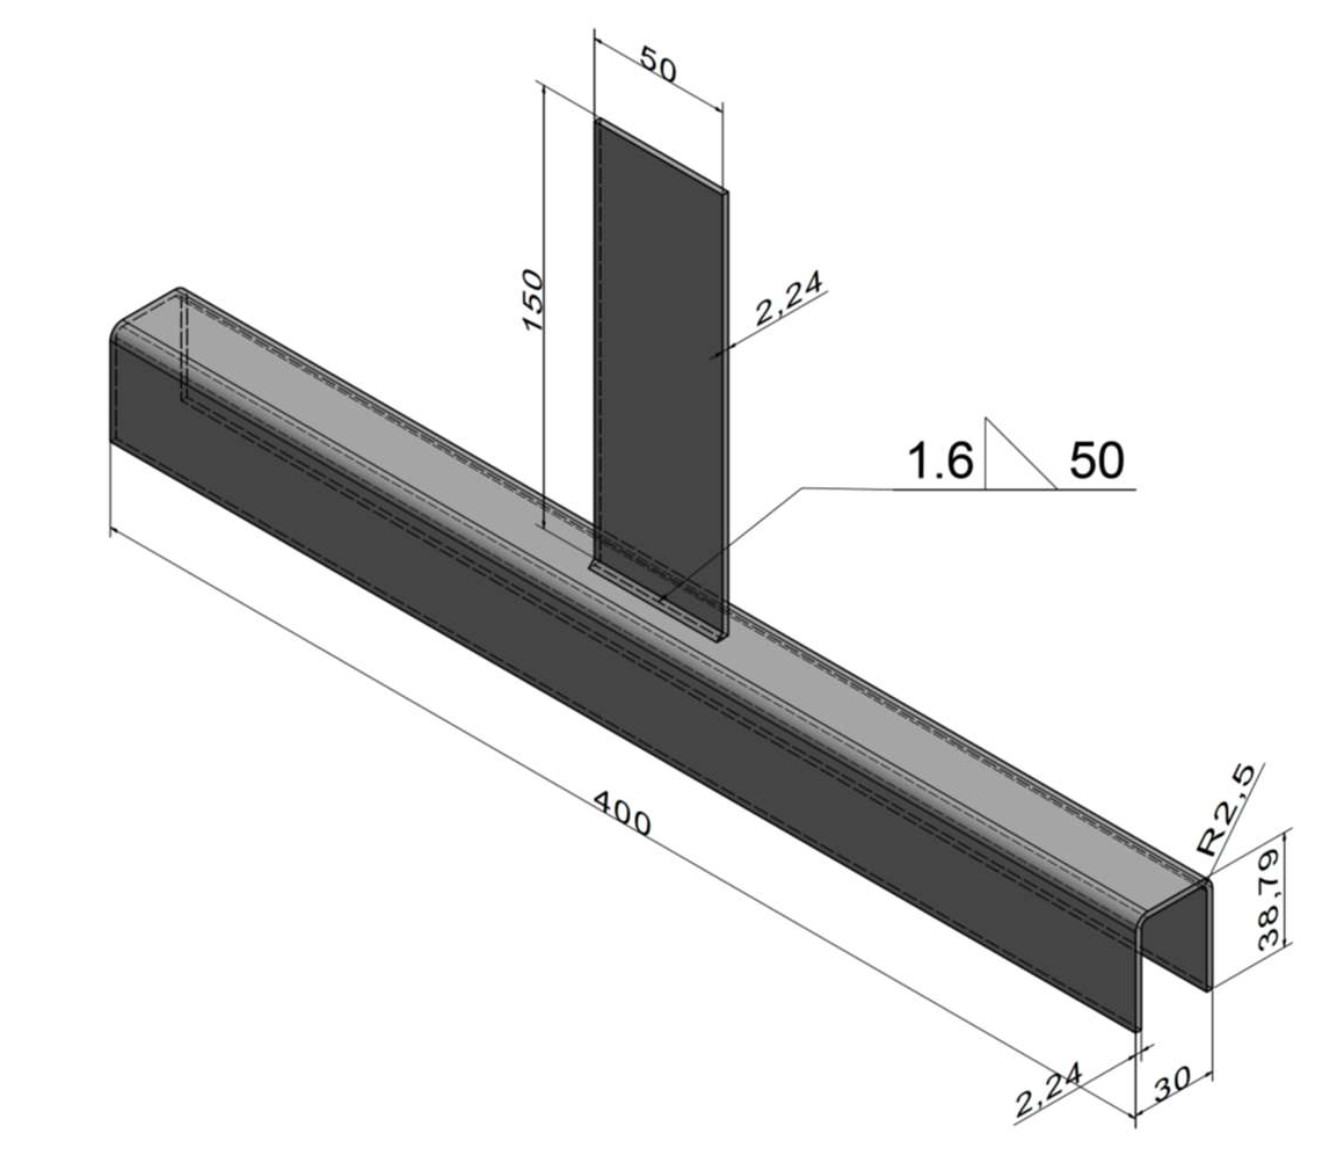
\includegraphics[width = 0.7\textwidth]{media/ditr.png}
    \caption{Συγκολλητή κατασκευή προς μελέτη.}
    \label{fig: ditr}
\end{figure}

Τα πειραματικά δεδομένα που έχουν δοθεί είναι για λόγο $R = 0$. Παρακάτω παρουσιάζονται τα δεδομένα για τον τύπο αστοχίας που φαίνεται στο \ref{fig:astoxia}. Όπως αναφέρθηκε και προηγουμένως, τα υπόλοιπα δύο δοκίμια και τα αποτελέσματα τους δεν λήφθηκαν υπόψη.
\par Για κάθε μία από τις μεθόδους, θα υπολογίζεται το εύρος τάσης για το κάθε δοκίμιο που ελέγχθηκε. Έπειτα, το έυρος αυτό θα συγκρίνεται με την αντίστοιχη καμπύλη διάρκειας ζωής σύμφωνα με τον οδηγό. Τα ζεύγη $(\Delta \sigma, N)$ που θα προκύπτουν θα αναφέρονται σε πιθανότητα επιβίωσης $50\%$. Επομένως, είναι αναγκαία και η μετατροπή σε πιθανότητα $97.7\%$ ώστε να μπορεί να γίνει η σύγκριση σύμφωνα με τον οδηγό IIW.

%pinakas dokimiws
\begin{table}[H]
    \centering
    \begin{tabular}{|c|c|c|c|}
        \hline
        \rowcolor{Dandelion}
        Spec No. & $F_m\; [kN]$ & $F_a\; [kN]$ & $N$\\
        \hline
        DI-01 & 28,2 & 27,9 & 89.000\\ \hline
        DI-02 & 37,6 & 37,3 & 29.000\\ \hline
        DI-03 & 34,2 & 33,9 & 41.000\\ \hline
        DI-04 & 31,2 & 30,9 & 73.000\\ \hline
        DI-05 & 40,2 & 39,9 & 23.000\\ \hline
        DI-06 & 22,1 & 22,0 & 190.000\\ \hline
        DI-08 & 18,1 & 18,0 & 603.000\\ \hline
        DI-09 & 20,1 & 20,0 & 453.000\\ \hline
        DI-10 & 21,1 & 21,0 & 575.000\\ \hline
        DI-11 & 26,2 & 26,0 & 167.000\\ \hline
        DI-12 & 16,5 & 16,4 & 1.470.000\\ \hline
        DI-13 & 23,2 & 23,0 & 335.000\\ \hline
        DI-15 & 24,2 & 24,0 & 246.000\\ \hline
    \end{tabular}
\end{table}
%morfh astoxias A

\begin{figure}[H]
    \centering
    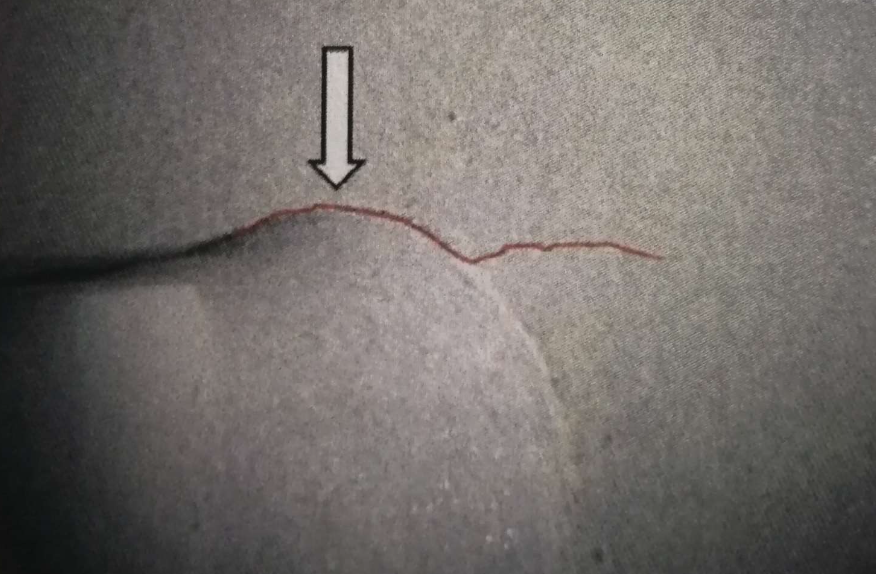
\includegraphics[width=0.5\linewidth]{media/astoxia.png}
    \caption{Μορφή αστοχίας πλειοψηφίας δοκιμίων.}
    \label{fig:astoxia}
\end{figure}

\subsection{Στατιστική ανάλυση}
Για τη δημιουργία της καμπύλης $97.7\%$ θα πρέπει να υπολογιστεί η τυπική απόκλιση $s$. Ορίζοντας ως:
\begin{align}
    \hat{y} &= log_{10} N\\
    \hat{x} &= log_{10} \Delta \sigma
\end{align}

Σύμφωνα με τους πίνακες της κανονικής κατανομής για να μετατραπούν τα σημεία στη ζητούμενη πιθανότητα αρκεί:
\begin{equation}
    \hat{y}_{97.7\%} = \hat{y}_{50\%} - 2.27s
\end{equation}

Από τα σημεία υπολογίζονται, κάθε φορά, οι συντελεστές $\alpha, \beta$ ως:
\begin{align}
    \beta &= \frac{\sum xy - \frac{\sum x \sum y}{n}}{\sum x^2 -n\overline{x}^2}\\
    \alpha &= \frac{\sum y}{n} - b\frac{\sum x}{n}
\end{align} 

Έπειτα, υπολογίζεται η τυπική απόκλιση ως:
\begin{equation}
    s = \sqrt{\frac{\sum (y(\overline{x}) - \overline{y})^2}{n}}
\end{equation}




\section{Υπολογισμοί συγκόλλησης}
\subsection{Μέθοδος Ονομαστικής Τάσης}
Για τη μέθοδο της ονομαστικής τάσης, αρκεί ο υπολογισμός των ονομαστικών τάσεων από τις φορτίσεις της κατασκευής. Αυτές σύμφωνα με τον οδηγό υπολογίζονται ως:
\begin{equation}
    \sigma = \frac{F}{A_w}
\end{equation}
Στη περίπτωση της δύναμης κάθετα προς τη ραφή της συγκόλλησης ο οδηγός IIW αναφέρει ότι η διατομή που χρησιμοποιείται εξαρτάται από μήκος της συγκόλλησης και το πάχος της ως:
\begin{equation}
    A_w = l\cdot a_w
\end{equation}
Στη περίπτωση προς μελέτη ωστόσο, η ραφή είναι παράλληλη προς την διεύθυνση της δύναμης. Έτσι, σαν διατομή συγκόλλησης επιλέγεται η διατομή της βάσης της συγκόλλησης (του κύριου τεμαχίου σε σχήμα Π). Τέλος, υπολογίζεται το εύρος τάσης για κάθε διαφορετικό δοκίμιο ως:
\begin{equation}
    \Delta \sigma = 2\cdot \frac{F_a}{A_w}
\end{equation}

Έχοντας υπολογίσει λοιπόν, τα σημεία $(\Delta \sigma, N)$, τα οποία εκφράζουν την $50\%$ πιθανότητα επιβίωσης, εξάγονται τα σημεία και για την $97.7\%$ πιθανότητα. Αυτό γίνεται, έτσι ώστε να συγκρίνονται όμοιες καμπύλες διάρκειας ζωής μεταξύ τους. Ο οδηγός αναφέρει ότι για την ανάλυση σε κόπωση με τη μέθοδο της ονομαστικής τάσης, πρέπει η καμπύλη διάρκειας ζωής να συγκριθεί με κάποια από τις τυποποιημένες καμπύλες FAT του οδηγού. Αρκεί λοιπόν, να επιλεχθεί η κατάλληλη κλάση FAT ώστε να εκτιμηθεί η διάρκεια ζωής της κατασκευής.
\par Σύμφωνα με τον οδηγό, η κλάση τυποποιημένης καμπύλης διάρκειας ζωής που βρίσκεται πιο κοντά στη παρόν περίπτωση είναι η \textit{FAT 71}. Το μήκος της συγκόλλησης είναι $50\; mm$
\subsection{Μέθοδος Κατασκευαστικής Τάσης}

\subsection{Μέθοδος Ενεργής Τάσης Εγκοπής}


\section{Συμπεράσματα}

\listoffigures
\listoftables

\end{document}